%%%%%%%%%%%%%%%%%%%%%%%%%%% asme2ej.tex %%%%%%%%%%%%%%%%%%%%%%%%%%%%%%
% ASME-format using LaTeX    										 %
% Written by   Do Quang Duy          								 %
%              Integration Engineering Laboratory                    %
%              Department of Military Academy Technology			 %
%              University of Viet Nam	                             %
%              PhaiVD, VN 1234                                       %
%              Tel: (083) 275-4691 (office)                          %
%                   (012) 345-6789 (lab)                             %
%              Fax: (012) 345-6789                                   %
%              Email: boycac0123@gmail.com                           %
%              WWW:   https://fig.mta.edu.vn				         %
%              Jun 24, 2010                                          %
% Modified: February 16, 2001 by Do Quang Duy	                     %
% Modified: January  01, 2003 by Do Quang Duy		                 %
% Use at your own risk, send complaints to /dev/null                 %
%%%%%%%%%%%%%%%%%%%%%%%%%%%%%%%%%%%%%%%%%%%%%%%%%%%%%%%%%%%%%%%%%%%%%%
\documentclass[twocolumn,10pt]{article}

\usepackage{natbib}
\usepackage{graphicx}
\usepackage{url}
\usepackage{indentfirst}
\graphicspath{ {./images/} }

\title{Fishing Websites Detection System}
%%% first author
\author{
	Do Quang Duy\\Cadet at\\Millitary Technology Academy\\University of Viet Nam\\Ha Noi, Viet Nam 12345\\
	\texttt{Email: boycac0123@gmail.com}
	\and
	Vu Dinh Phai\\Professor at\\Millitary Technology Academy\\University of Viet Nam\\Ha Noi, Viet Nam 12345\\
	\texttt{Email: phaivd@gmail.com}
}


\begin{document}
\maketitle
%%%%%%%%%%%%%%%%%%%%%%%%%%%%%%%%%%%%%%%%%%%%%%%%%%%%%%%%%%%%%%%%%%%%%%

\begin{abstract}
\textbf{The result of our project is to build a machine
learning clarification on the problem of identifying fishing websites. The end target of our project will be software that uses a machine-learning algorithm to recognize fishing URLs. Fishing is the method of obtaining user credentials and sensitive data from users by pretending as a good website. In fishing, the user is given a
reflector website that is alike to the legitimate one but with
malicious code to obtain and give user credentials to fishers.
It can lead to large economic wounds for customers
of banking and commercial services. We plan to solve these challenges by using many machine learning classification algorithms to classify and then comparing these algorithms' performance on our dataset. We will use SVM, Decision Trees, and Neural Networks, the dataset of the fishing websites from the UCI Machine Learning repository, and select the most suitable model to produce a browser plugin, which can be distributed as a chrome extension.}
\end{abstract}
%%%%%%%%%%%%%%%%%%%%%%%%%%%
\section{Introduction}

An important challenge in the network security field is providing a power Fishing Website Detection System (FWDS). The modern approach is using machine learning techniques to solve the challenges. The advance for this solution includes high accuracy (and minimum costs), less effort in finding available training data, a reusable model, and plenty of machine learning architecture. But the present models still have a normal accuracy, that such models lead to ineffectual and unstable detection.	

Two major limitations are considered about this challenge. First, the rapid increase in the number of websites and users with less security knowledge, and will continue to increase in the future. The popularity of the Internet,  the necessity of websites in business and life, the low cost on the Internet and increase the income of resident is the reason. Therefore we need a technique that can determine normal and fishing websites in a drastic growth, effectual and stable manner. Second, the plenty of different types of fishing websites on the internet, and it will increase in the future. This is considered an important challenge and makes hardly when to try to determine normal and fishing websites. It decreases the accuracy and stability of building a model for website detection.

Recently, one of the modern approach attention in detect fishing websites has been the application of machine learning techniques such as Support Vector Machines (SVM), Neural Network (NN), Random Forest (RF) [1]. Although these techniques have to lead to improvements in detection accuracy. However, these techniques still have some limitations, like the less accuracy in predict model, unclear and small training data, inefficient features. This cost a lot of effort to training and process but it is unacceptable and has a high error percent [2]. Therefore, this is not satisfying for a dynamic and asynchronous environment.

From the limitations, a method to solve the challenge of machine learning, a new method of extracting features, which can handle some of the limitations. Machine learning has the ability to work with insufficient knowledge[3]. It can make a deep automatic analysis of websites and faster determine the fishing websites.
In this paper, we suggest a machine learning model for active FWDS operation within the internet. The model we suggest is modern in machine learning, that able to correctly analyzing almost all websites. -More specifically, we use the advanced power model, find a new set of features. We have practically evaluated our model using functions from the library on the website's datasets. These datasets also have some limitations but they remain popularly-used standard within the similar product so that we can compare to others products.
This paper distributes these new contributions:

- A new machine learning model, a modern model, can increase the accuracy of the classification model. We have demonstrated on benchmark websites dataset is when using this machine learning model, the accuracy of the classification algorithm can grow from 1.5\% to 4.5\%.

- The rest of this paper is structure as follows. Section 2 presents relevant background information. Section 3 examines existing research. Section 4 specifies our proposed solution, which is subsequently evaluated in Section 5. Section 6 discusses our findings from the evaluation. Finally, the paper concludes in Section 7.
%%%%%%%%%%%%%%%%%%%%%%%%%%%%%%%%%%%%%%%%%%%%%%%%%%%%%%%%%
\section{Related work}

We propose two approaches to detect fishing websites that are using a blacklist and evaluating the source code to check for features commonly related to fishing websites. The first approach, using a blacklist need to maintain a publicly available list of reported fishing sites, the advance this approach is that keep the number of victims of any new fishing websites very low, but this approach has a big problem that it requires new fishing websites has to be detected first before it can be reported. As fishing techniques become more intelligent and delicate, it will be harder to detect new fishing websites. 	 
The other approach evaluates the source code to extract features of the websites, from that we can determine a website is normal or fishing within a minute, this approach is better than using a blacklist since we can potentially detect a new fishing website. However, as said before, because of the plenty of different methods of fishing websites and it will increase in the future, fishing website detection has become more difficult. 

Commonly, evaluating the website's source code is related to maintain several identified fishing attributes. These make it hard for the fishing detection system to determine a new fishing pattern. Therefore, machine learning is a good choice, when a new fishing pattern is discovered, it relearns from the data to detect it.
%%%%%%%%%%%%%%%%%%%%%%%%%%%%%%%%%%%%%%%%%%%%%%%%%%%%%%%%%
\section{Propose approach}

We recommend using machine learning to overwhelm the disadvantages related to the common methods of fishing detection. A fishing detection candidate needs to satisfy the machine learning application solutions as the huge data on fishing websites patterns. The primary plan is to use machine learning algorithms on a possible dataset of the fishing website to create a form that can be used to produce classifications in real-time if a provided website is fishing or a valid website. We expect to provide the trained model into a software application that can be used easily by end-users for fighting fishing attempts. We have decided to execute a machine learning algorithm from scratch using JavaScript and develop a Chrome extension with it for this goal. That will allow us to implement the trained model simply on the Chrome Web Store, everyone can download and use our product for fishing detection. 

There are three requirements that we need to considered when deciding the machine learning algorithm for our product. First, the trained model must have high accuracy, because a product is deployed to the end-users in the real world should not return bad results. Second, the classification algorithm in real-time is necessary. It should have a very low execution time and also use less computational resources. Third, we consider two important scores false positives and false negatives when choosing a machine learning algorithm for the problem of fishing detection. This allows a user, not to wrongly access a fishing website. Therefore, we look at these three requirements when selecting our phishing detection classifier.

We used the ‘Fishing Websites Dataset’ from the UCI Machine learning repository to estimate our machine learning techniques. It has 11,055 URLs (websites) with 6157 fishing cases and 4898 legitimate cases. Each case has 30 features. Each feature is connected with a rule. It is termed fishing if the rule satisfies. The opposite is termed as legitimate. The features get three values returned. If the rule is satisfied then return 1 if the rule is partially satisfied then return 0 if the rule is not satisfied then return -1. We used the training dataset from the "Phishing Websites Data Set" of the UCI Machine learning repository for our project. The dataset has 11,055 instances consist of 6157 fishing cases and 4898 legitimate cases. There are 30 features containing various attributes each instance typically connected with fishing, suspicious or legitimate as the appearance of IP address in the URL domain or the appearance of JavaScript code to change the web browser address bar information. Every feature is connected with a rule.

If the rule is satisfied, it is in terms of fishing and legitimate otherwise. We normalized the dataset to include only discrete values. Each feature of each instance will include 1 if the rule associated with that feature is satisfied, 0 if partially satisfied, and -1 if unsatisfied.

We classified the training dataset by the features into four categories:

i) Address Bar based Features

ii) Abnormal Based Features

iii) HTML and JavaScript based Features

iv) Domain based Features
%%%%%%%%%%%%%%%%%%%%%%%%%%%%%%%%%%%%%%%%%%%%%%%%%%%%%%%%%%%%%%%%%%%%%%	
\subsection{Address Bar based Features}
%%%%%%%%%%%%%%%%%%%%%%%%%%%%%%%%%%%%%%%%%%%%%%%%%%%%%%%%%%%%%%%%%%%%%%
\subsubsection{Using the IP Address}

If an IP address is used as an alternative of the domain name in the URL, such as “http://125.98.3.123/fake.html”, users can be sure that someone is trying to steal their personal information. Sometimes, the IP address is even transformed into hexadecimal code as shown in the following link http://0x58.0xCC.0xCA.0x62/2/paypal.ca/index\\.html

\begin{center}
\it Rule:
\fbox{\fbox{\parbox{3in}{\centering If The Domain Part has an IP Address→Fishing\\Otherwise→Legitimate}}}
\end{center}

\subsubsection{Long URL to Hide the Suspicious Part}

Phishers can use long URL to hide the doubtful part in the address bar. For example:

http://federmacedoadv.com.br/3f/aze/ab51e2e319e\\51502f416dbe46b773a5e/?cmd=\_home\&amp;dispatch\\=11004d58f5b74f8dc1e7c2e8dd4105e811004d58f5b74f\\8dc1e7c2e8dd4105e8@phishing.website.html

To ensure accuracy of our study, we calculated the length of URLs in the dataset and produced an average URL length. The results showed that if the length of the URL is greater than or equal 54 characters then the URL classified as phishing. By reviewing our dataset we were able to find 1220 URLs lengths equals to 54 or more which constitute 48.8\% of the total dataset size.

\begin{center}
\it Rule:
\fbox{\fbox{\parbox{3in}{\centering URLlength<54$\rightarrow$feature=Legitimate 
\\elseif URLlength$\geq$54$\cap$$\leq$75$\rightarrow$feature=Suspicious  otherwise$\rightarrow$feature=Fishing
}}}
\end{center}

We have been able to update this feature rule by using a method based on frequency and thus improving upon its accuracy.
%%%%%%%%%%%%%%%%%%%%%%%%%%%%%%%%%%%%%%%%%%%%%%%%%%
\subsubsection{Using URL Shortening Services “TinyURL”}

URL shortening is a method on the “World Wide Web” in which a URL may be made considerably smaller in length and still lead to the required webpage. This is accomplished by means of an “HTTP Redirect” on a domain name that is short, which links to the webpage that has a long URL. For example, the URL http://portal.hud.ac.uk/ can be shortened to “bit.ly/19DXSk4”.
\begin{center}
\it Rule:
\fbox{\fbox{\parbox{2.5in}{\centering TinyURL$\rightarrow$Fishing \\Otherwise$\rightarrow$Legitimate
}}}
\end{center}
%%%%%%%%%%%%%%%%%%%%%%%%%%%%%%%%%%%%%%%%%%%%%%%%%%
\subsubsection{URL have @ Symbol}
Using “@” symbol in the URL leads the browser to ignore everything preceding the “@” symbol and the real address often follows the “@” symbol. 
\begin{center}
\it Rule:
\fbox{\fbox{\parbox{2.5in}{\centering URL have @ Symbol$\rightarrow$Fishing \\Otherwise$\rightarrow$Legitimate
}}}
\end{center}
%%%%%%%%%%%%%%%%%%%%%%%%%%%%%%%%%%%%%%%%%%%%%%%%%%
\subsubsection{Redirecting using //}

The existence of “//” within the URL path means that the user will be redirected to another website. An example of such URL’s is: “http://www.legitimate.com//http://www.phishing\\.com”. We examin the location where the “//” appears. We find that if the URL starts with “HTTP”, that means the “//” should appear in the sixth position. However, if the URL employs “HTTPS” then the “//” should appear in seventh position.
\begin{center}
\it Rule:
\fbox{\fbox{\parbox{3in}{\centering The Position of the Last Occurrence of // in URL$ >$7$\rightarrow$Fishing\\Otherwise$\rightarrow$Legitimate
}}}
\end{center}
%%%%%%%%%%%%%%%%%%%%%%%%%%%%%%%%%%%%%%%%%%%%%%%%%%
\subsubsection{Adding Prefix or Suffix Separated by (-) to the Domain}

The dash symbol is rarely used in legitimate URLs. Phishers tend to add prefixes or suffixes separated by (-) to the domain name so that users feel that they are dealing with a legitimate webpage. For example http://www.Confirme-paypal.com/.
\begin{center}
\it Rule:
\fbox{\fbox{\parbox{2.5in}{\centering URL have - symbol$\rightarrow$Fishing\\Otherwise$\rightarrow$Legitimate
}}}
\end{center}
%%%%%%%%%%%%%%%%%%%%%%%%%%%%%%%%%%%%%%%%%%%%%%%%%%
\subsubsection{Sub Domain and Multi Sub Domains}

Let us assume we have the following link: http://www.hud.ac.uk/students/. A domain name might include the country-code top-level domains (ccTLD), which in our example is “uk”. The “ac” part is shorthand for “academic”, the combined “ac.uk” is called a second-level domain (SLD) and “hud” is the actual name of the domain. To produce a rule for extracting this feature, we firstly have to omit the (www.) from the URL which is in fact a sub domain in itself. Then, we have to remove the (ccTLD) if it exists. Finally, we count the remaining dots. If the number of dots is greater than one, then the URL is classified as “Suspicious” since it has one sub domain. However, if the dots are greater than two, it is classified as “Phishing” since it will have multiple sub domains. Otherwise, if the URL has no sub domains, we will assign “Legitimate” to the feature.  
\begin{center}
\it Rule:
\fbox{\fbox{\parbox{2.5in}{\centering Dots of domain part=1$\rightarrow$Legitimate\\Dots of domain part=2$\rightarrow$Suspicious\\Otherwise$\rightarrow$Fishing
}}}
\end{center}
%%%%%%%%%%%%%%%%%%%%%%%%%%%%%%%%%%%%%%%%%%%%%%%%%%
\subsubsection{HTTPS (Hyper Text Transfer Protocol with Secure Sockets Layer)}

The existence of HTTPS is very important in giving the impression of website legitimacy, but this is clearly not enough. The authors in (Mohammad, Thabtah and McCluskey 2012) (Mohammad, Thabtah and McCluskey 2013) suggest checking the certificate assigned with HTTPS including the extent of the trust certificate issuer, and the certificate age. Certificate Authorities that are consistently listed among the top trustworthy names include: “GeoTrust, GoDaddy, Network Solutions, Thawte, Comodo, Doster and VeriSign”. Furthermore, by testing out our datasets, we find that the minimum age of a reputable certificate is two years.
\begin{center}
	\it Rule:
	\fbox{\fbox{\parbox{3in}{\centering Use https$\cap$Issuer is Trusted$\cap$Age of Certificate$\geq$1 Year$\rightarrow$Legitimate\\Using https$\cap$Issuer is not Trusted $\rightarrow$Suspicious\\Otherwise$\rightarrow$Fishing
	}}}
\end{center}
%%%%%%%%%%%%%%%%%%%%%%%%%%%%%%%%%%%%%%%%%%%%%%%%%%
\subsubsection{Domain Registration Length}

Based on the fact that a phishing website lives for a short period of time, we believe that trustworthy domains are regularly paid for several years in advance. In our dataset, we find that the longest fraudulent domains have been used for one year only. 
\begin{center}
	\it Rule:
	\fbox{\fbox{\parbox{2.5in}{\centering Domains Expireson$\leq$1 years$\rightarrow$Fishing\\Otherwise$\rightarrow$Legitimate
	}}}
\end{center}
%%%%%%%%%%%%%%%%%%%%%%%%%%%%%%%%%%%%%%%%%%%%%%%%%%
\subsubsection{Favicon}

A favicon is a graphic image (icon) associated with a specific webpage. Many existing user agents such as graphical browsers and newsreaders show favicon as a visual reminder of the website identity in the address bar. If the favicon is loaded from a domain other than that shown in the address bar, then the webpage is likely to be considered a Phishing attempt. 
\begin{center}
	\it Rule:
	\fbox{\fbox{\parbox{3in}{\centering Favicon Loaded External Domain$\rightarrow$Fishing\\Otherwise$\rightarrow$Legitimate
	}}}
\end{center}
%%%%%%%%%%%%%%%%%%%%%%%%%%%%%%%%%%%%%%%%%%%%%%%%%%
\subsubsection{Using Non-Standard Port}

This feature is useful in validating if a particular service (e.g. HTTP) is up or down on a specific server. In the aim of controlling intrusions, it is much better to merely open ports that you need. Several firewalls, Proxy and Network Address Translation (NAT) servers will, by default, block all or most of the ports and only open the ones selected. If all ports are open, phishers can run almost any service they want and as a result, user information is threatened. The most important ports and their preferred status are shown in Table 2. 
\begin{center}
\it Rule:
\fbox{\fbox{\parbox{2.5in}{\centering Port \# is of the Prefer Status$\rightarrow$Fishing\\Otherwise$\rightarrow$Legitimate }}}
\end{center}
\begin{center}
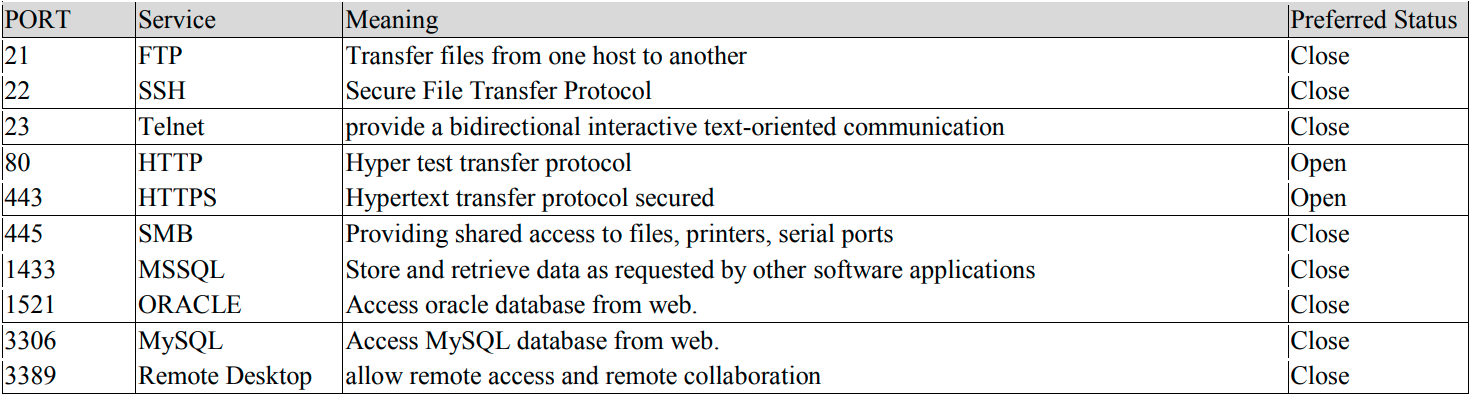
\includegraphics[scale=0.15]{port}
\end{center}
%%%%%%%%%%%%%%%%%%%%%%%%%%%%%%%%%%%%%%%%%%%%%%%%%%
\subsubsection{The Existence of “HTTPS” Token in the Domain Part of the URL}

The phishers may add the “HTTPS” token to the domain part of a URL in order to trick users. For example,
http://https-www-paypal-it-webapps-mpp-home.soft-hair.com/.
\begin{center}
\it Rule:
\fbox{\fbox{\parbox{2.5in}{\centering Using HTTPToken Duy DomainPartofTheURL $\rightarrow$Fishing\\Otherwise$\rightarrow$Legitimate
}}}
\end{center}
%%%%%%%%%%%%%%%%%%%%%%%%%%%%%%%%%%%%%%%%%%%%%%%%%%
\subsection{Abnormal Based Features}
%%%%%%%%%%%%%%%%%%%%%%%%%%%%%%%%%%%%%%%%%%%%%%%%%%%%%%%%%%%%%%%%%%%%%%
\subsubsection{Request URL}

Request URL examines whether the external objects contained within a webpage such as images, videos and sounds are loaded from another domain. In legitimate webpages, the webpage address and most of objects embedded within the webpage are sharing the same domain. 
\begin{center}
\it Rule:
\fbox{\fbox{\parbox{3in}{\centering \% of Request URL$<$22\% $\rightarrow$Legitimate\\\% of Request URL$\geq$22\%$\cap$$\leq$61\%$\rightarrow$Suspicious\\Otherwise$\rightarrow$Fishing
}}}
\end{center}
%%%%%%%%%%%%%%%%%%%%%%%%%%%%%%%%%%%%%%%%%%%%%%%%%%
\subsubsection{URL of Anchor}

An anchor is an element defined by the $ < $a$ > $ tag. This feature is treated exactly as “Request URL”. However, for this feature we examine:

1. If the $ < $a$ > $ tags and the website have different domain names. This is similar to request URL feature. 

2. If the anchor does not link to any webpage, e.g.:

A. $<$a href=“\#”$>$

B. $<$a href=“\#content”$>$

C. $<$a href=“\#skip”$>$

D. $<$ a href=“JavaScript ::void(0)”$>$
\begin{center}
\it Rule:
\fbox{\fbox{\parbox{3in}{\centering \% URL of Anchor$<$31\% $\rightarrow$Legitimate\\\% URL of Anchor$\geq$31\%$\cap$$\leq$67\%$\rightarrow$Suspicious\\Otherwise$\rightarrow$Fishing
	}}}
\end{center}
%%%%%%%%%%%%%%%%%%%%%%%%%%%%%%%%%%%%%%%%%%%%%%%%%%
\subsubsection{temp}
\begin{center}
	\it Rule:
	\fbox{\fbox{\parbox{2.5in}{\centering $\rightarrow$Fishing\\Otherwise$\rightarrow$Legitimate
	}}}
\end{center}%%%%%%%%%%%%%%%%%%%%%%%%%%%%%%%%%%%%%%%%%%%%%%%%%%
\subsubsection{Links in <Meta>, <Script> and <Link> tags}

Given that our investigation covers all angles likely to be used in the webpage source code, we find that it is common for legitimate websites to use <Meta> tags to offer metadata about the HTML document; <Script> tags to create a client side script; and <Link> tags to retrieve other web resources. It is expected that these tags are linked to the same domain of the webpage. 
\begin{center}
\it Rule:
\fbox{\fbox{\parbox{3in}{\centering \% of Links in "$<$Meta$ > $","$ < $Script$ > $" and "$ < $Link$ > $"$ < $17\%→ Legitimate\\\% of Links in " $ < $ Meta $ > $ "," $ < $ Script $ > $ " and " $ < $ Link$ > $"  $\geq$ 17 
$\cap$$\leq$81\% → Suspicious\\Otherwise$\rightarrow$Fishing
}}}
\end{center}%%%%%%%%%%%%%%%%%%%%%%%%%%%%%%%%%%%%%%%%%%%%%%%%%%
\subsubsection{Server Form Handler (SFH)}

SFHs that contain an empty string or “about:blank” are considered doubtful because an action should
be taken upon the submitted information. In addition, if the domain name in SFHs is different from
the domain name of the webpage, this reveals that the webpage is suspicious because the submitted
information is rarely handled by external domains
\begin{center}
\it Rule:
\fbox{\fbox{\parbox{3in}{\centering SFH is "about: blank" Or Is Empty → Fishing\\SFH Refers To A Different Domain → Suspicious\\Otherwise → Legitimate
}}}
\end{center}%%%%%%%%%%%%%%%%%%%%%%%%%%%%%%%%%%%%%%%%%%%%%%%%%%
\subsubsection{Submitting Information to Email}
Web form allows a user to submit his personal information that is directed to a server for processing.
A phisher might redirect the user’s information to his personal email. To that end, a server-side script
language might be used such as “mail()” function in PHP. One more client-side function that might be
used for this purpose is the “mailto:” function. 
\begin{center}
\it Rule:
\fbox{\fbox{\parbox{2.5in}{\centering Using "mail()" or "mailto:" Function to Submit User Information → Fishing \\Otherwise$\rightarrow$Legitimate
}}}
\end{center}
%%%%%%%%%%%%%%%%%%%%%%%%%%%%%%%%%%%%%%%%%%%%%%%%%%
\subsubsection{Abnormal URL}

This feature can be extracted from WHOIS database. For a legitimate website, identity is typically
part of its URL
\begin{center}
	\it Rule:
	\fbox{\fbox{\parbox{3in}{\centering Host Name Is Not Included In URL→Fishing\\Otherwise$\rightarrow$Legitimate
	}}}
\end{center}
%%%%%%%%%%%%%%%%%%%%%%%%%%%%%%%%%%%%%%%%%%%%%%%%%%
\subsection{HTML and JavaScript based Features}
%%%%%%%%%%%%%%%%%%%%%%%%%%%%%%%%%%%%%%%%%%%%%%%%%%%%%%%%%%%%%%%%%%%%%%
\subsubsection{IFrame Redirection}

IFrame is an HTML tag used to display an additional webpage into one that is currently shown.
Phishers can make use of the “iframe” tag and make it invisible i.e. without frame borders. In this
regard, phishers make use of the “frameBorder” attribute which causes the browser to render a visual
delineation. 
\begin{center}
\it Rule:
\fbox{\fbox{\parbox{2.5in}{\centering Using iframe→Fishing\\Otherwise$\rightarrow$Legitimate
}}}
\end{center}
%%%%%%%%%%%%%%%%%%%%%%%%%%%%%%%%%%%%%%%%%%%%%%%%%%
\subsection{Domain based Features}
%%%%%%%%%%%%%%%%%%%%%%%%%%%%%%%%%%%%%%%%%%%%%%%%%%%%%%%%%%%%%%%%%%%%%%
\subsubsection{Age of Domain}

This feature can be extracted from WHOIS database (Whois 2005). Most phishing websites live for a short period of time. By reviewing our dataset, we find that the minimum age of the legitimate domain is 6 months. 
\begin{center}
\it Rule:
\fbox{\fbox{\parbox{3in}{\centering Age Of the Domain$\geq$6 months → Legitimate\\Otherwise$\rightarrow$Fishing
}}}
\end{center}
%%%%%%%%%%%%%%%%%%%%%%%%%%%%%%%%%%%%%%%%%%%%%%%%%%
\subsubsection{DNS Record}
For phishing websites, either the claimed identity is not recognized by the WHOIS database (Whois 2005) or no records founded for the hostname (Pan and Ding 2006). If the DNS record is empty or not found then the website is classified as “Phishing”, otherwise it is classified as “Legitimate”. 
\begin{center}
\it Rule:
\fbox{\fbox{\parbox{3in}{\centering no DNS Record For the Domain$\rightarrow$Fishing\\Otherwise$\rightarrow$Legitimate
}}}
\end{center}
%%%%%%%%%%%%%%%%%%%%%%%%%%%%%%%%%%%%%%%%%%%%%%%%%%
\subsubsection{Website Traffic}

This feature measures the popularity of the website by determining the number of visitors and the number of pages they visit. However, since phishing websites live for a short period of time, they may not be recognized by the Alexa database (Alexa the Web Information Company., 1996). By reviewing our dataset, we find that in worst scenarios, legitimate websites ranked among the top 100,000. Furthermore, if the domain has no traffic or is not recognized by the Alexa database, it is classified as “Phishing”. Otherwise, it is classified as “Suspicious”. 
\begin{center}
	\it Rule:
	\fbox{\fbox{\parbox{2.5in}{\centering Website Rank < 100,000 → Legitimate\\Website Rank > 100,000 → Suspicious\\Otherwise$\rightarrow$Fishing
	}}}
\end{center}
%%%%%%%%%%%%%%%%%%%%%%%%%%%%%%%%%%%%%%%%%%%%%%%%%%
\subsubsection{Google Index}

This feature examines whether a website is in Google’s index or not. When a site is indexed by
Google, it is displayed on search results (Webmaster resources, 2014). Usually, phishing webpages
are merely accessible for a short period and as a result, many phishing webpages may not be found on
the Google index
\begin{center}
\it Rule:
\fbox{\fbox{\parbox{2.5in}{\centering Webpage Indexed by Google → Legitimate\\Otherwise$\rightarrow$Fishing
	}}}
\end{center}
%%%%%%%%%%%%%%%%%%%%%%%%%%%%%%%%%%%%%%%%%%%%%%
\subsubsection{Statistical-Reports Based Feature}
Several parties such as PhishTank (PhishTank Stats, 2010-2012), and StopBadware (StopBadware,
2010-2012) formulate numerous statistical reports on phishing websites at every given period of time;
some are monthly and others are quarterly. In our research, we used 2 forms of the top ten statistics
from PhishTank: “Top 10 Domains” and “Top 10 IPs” according to statistical-reports published in the
last three years, starting in January2010 to November 2012. Whereas for “StopBadware”, we used
“Top 50” IP addresses.
\begin{center}
\it Rule:
\fbox{\fbox{\parbox{3in}{\centering Host Belongs to Top Fishing IPs or Top Fishing Domains→Fishing\\Otherwise$\rightarrow$Legitimate
}}}
\end{center}


\end{document}